\documentclass{article}

\usepackage{times}
\usepackage{graphicx}
\usepackage{subfigure}
\usepackage{natbib}
\usepackage{algorithm}
\usepackage{algorithmic}
\usepackage{lipsum}
\usepackage{todonotes}
\usepackage {mathtools}
\usepackage{amsthm}
\usepackage{amsmath}
\usepackage[accepted]{icml2017}
\icmltitlerunning{CS 281 Final Project Template}

\begin{document}

\twocolumn[
\icmltitle{Latent Variable Matrix Factorization in Heterogeneous Peer Prediction}
\begin{icmlauthorlist}
\icmlauthor{Brian Hentschel}{}
  \icmlauthor{Anna S. Hilgard}{}
\icmlauthor{Casey Meehan}{}
\end{icmlauthorlist}

\vskip 0.3in
]

\begin{abstract}
In the setting of heterogeneous peer prediction, soliciting truthful reporting from agent's is done via learning an agent's reporting type. This learned reporting type is used to produce payout schemes such that telling the truth is a low-regret strategy. Mostly, this work is done via clustering on user-user $\Delta$ matrices, which capture dependence in the probability of user's reports.

In this paper, we present advantages to using latent variable matrix factorization in heterogeneous peer prediction. 
We show that clustering users by their corresponding latent variables is enough to produce a good clustering when comparing user's $\Delta$ Matrices. Additionally, we show that it is orders of magnitude faster to produce these clusterings when using a latent variable representation. Finally, we show how latent variables and non-task data can be used in conjunction to produce solutions for the cold start problem, where a user has no report data and thus has an unknown initial reporting strategy.
  \begin{itemize}
  \item This document describes the expected style, structure, and rough proportions for your final project write-up.
  \item While you are free to break from this structure, consider it a strong prior for our expectations of the final report.
\item Length is a hard constraint. You are only allowed max \textbf{8 pages} in this format. While you can include supplementary material, it will not be factored into the grading process. It is your responsibility to convey the main contributions of the work in the length given.
  \end{itemize}


\lipsum[1]
\end{abstract}

\section{Introduction}
\label{sec:introduction}

%Example Structure:
%\begin{itemize}
%\item What is the problem of interest and what (high-level) are the current best methods for solving it?
%\item How do you plan to improve/understand/modify this or related methods?
%\item Preview your research process, list the contributions you made, and summarize your experimental findings.
%\end{itemize}

In peer prediction settings with heterogeneous users, the goal is to make truthful reporting a low-regret strategy for any agent. To fully minimize expected regret while allowing for heterogeneity, this would require the computation and use of individualized user-user signal correlations for every pair of users. This is in general computationally infeasible, so methodologies typically focus instead on clustering similar users while trying to minimally distort their individual signal distributions. 

Additionally, because this method explicitly requires an existing signal distribution, there is a cold start problem: if we do not already have a significant amount of task data for a new user, we cannot know how properly to reward them in comparison to their peers. In our project, we focus on two specific goals:
\begin{enumerate}
\item Clustering is usually done by comparing each user`s reports with other users. We aim to speed up this clustering by using latent variable matrix factorization and then clustering on much smaller latent variables.
\item Bootstrapping the clustering process by using non-task data to form an initial clustering before agent reporting begins.
\end{enumerate}

\section{Background and Related Work}\label{sec:Background}
%Example Structure:
%\begin{itemize}
%\item What information does a non-expert need to know about the problem domain?
%\item What data exists for this problem?
%\item What are the challenges/opportunities inherent to the data? (High dimensional, sparse, missing data, noise, structure, discrete/continuous, etc?)
%\end{itemize}

In \citet{shnayder2016informed}, Shnayder et al. prove that the Correlated Agreement multi-task peer prediction mechanism maximally incentivizes truthful reporting without a ground truth for homogeneous users. The CA mechanism can be generalized to non-homogeneous users but requires a prohibitive number of user reports; thus, \citet{agarwal2017} bounds expected regret by clustering users with similar signal-report distributions.  This regret bound is proportional to the L1 difference between user-user '$\Delta$ Matrices' and those of their respective clusters, where a $\Delta$ Matrix of users $q,r$ is defined as: 
\begin{align*}
D_{q,r}(i,j) &= p(\textrm{q reports i, r reports j}) \\
&- p(\textrm{q reports i})p(\textrm{r reports j})
\end{align*}

As far as we know, \citep{agarwal2017} is the only paper to specifically consider clustering methods for heterogeneous peer prediction. The paper differs from our work in that it assumes all of the relevant data exists and seeks to prove a theoretical upper bound on regret rather than to study empirical average regret in settings with sparse data. To demonstrate this, the authors restrict their dataset to a small subset of only those users for whom there is a full joint distribution between any two users, resulting in only 269 users. 

Further, while the authors prove a theoretical bound in the case of empirically estimated ground truth, the tests they run on real data rely on the existence of a known ground truth label. This allows them to calculate individual signal confusion matrices using methods developed in \citet{dawid1979maximum} and leverage tensor decomposition techniques from \citet{anandkumar2014tensor} and \citet{zhang2016spectral} to compute average clusters directly. We seek to show that in the more general case of incomplete data with no ground truth labels, clustering instead on user-specific latent variables learned through matrix factorization can lead to similar computational savings as tensor decomposition while eliminating the need for labels.  Further, we show that these computationally efficient clusterings are similarly effective with respect to incentivizing truthfulness as clustering on $\Delta$ matrices directly.

The use of the Correlated Agreement mechanism \citep{shnayder2016informed} requires that the $\Delta$ matrices are already known or can be empirically estimated from user reports. However, in practice, newly introduced users have contributed no reports and thereby cannot be clustered accurately. While nothing in the peer prediction literature addresses this cold start problem, it is well studied in the field of matrix factorization. The most similar method to ours, in that it incorporates non-task data, is \citep{kula2015metadata}. 


\section{Datasets}
\subsection{Task Data}
The primary dataset we use is that of the \emph{Good Judgment Global Forecasting Competition}, available at \texttt{https://dataverse.harvard.edu/dataverse.}
\texttt{xhtml?alias=gjp}. There are many challenges inherent to this dataset. First, the idea of a task is not well-defined. Users enter predictions in continuous time, and the true probability of an event will change over time, such that each minute could be considered a different task (Note that if we expect users to only update their predictions in response to new information, these time-question tasks will be independent conditional on the signal). We choose to bucket these responses by week to mediate between the desire to allow for variation in true probability over time while maintaining sufficient task response density. This results in 1,499,294 predictions by 2,052 users on 1,548 tasks. Secondly, the signal itself can be expected to have a high degree of noise, as the probability of any of these global events is not well-defined even in the absence of individual interpretation effects. 

To study the effects of the clustering methodologies in a slightly less noisy realm, we additionally use a second dataset of user judgments on whether or not websites contained adult content. This dataset, termed \emph{Adult}, was pulled from the Square Project at the University of Texas. The data is available at \texttt{https://github.com/ipeirotis/}
\texttt{Get-Another-Label/tree/master/data}. We limit the dataset to users who gave at least one report of each signal, resulting in 65,144 reports by 389 users on 10,381 tasks.

Both datasets required significant preprocessing to account for sparsity of signal distributions and to compute the $\Delta$ matrices. Additionally, because Good Judgment reports were continuous rather than discrete, we bucketed the responses into five uniform bins, which we use to compute the matrices.

\subsection{Non-Task Data}
In addition to user predictions (task data), the Good Judgement dataset includes a variety of questions to assess the knowledge and ability of each user as well as their psychological and characteristic makeup. For instance, questions to assess knowledge might ask them about world events or to solve a moth problem. Questions about character might ask them to state on a scale from 1-7 how just they believe the world is. We then use this non-task data to address the cold start problem discussed in section 2. 

The psychological data contains both binary and ordinal features. A binary feature may be an answer to a 'yes/no' question or whether the user correctly answered a diagnostic math test question. An ordinal feature captures some continuous measure of that user's character, \textit{e.g.} user age or weekly workhours. To discretize ordinal features, we bucket each into a finite set of uniform bins similar to the Good Judgement report data. However, the number of bins is feature-dependent. 

The dataset consists of 168 features for each of the 2052 users. There are a significant number of missing answers in the dataset. For binary features, we made negative answers into $-1$, missing answers into $0$, and positive answers into $1$. For ordinal features, we filled NaNs in with the average value of that feature. {\color{red} Talk about data cleaning here?}

%\section{Related Work}
%
%%Example Structure:
%%\begin{itemize}
%%\item What 3-5 papers have been published in this space?
%%\item How do these  differ from your approach?
%%\item What data or methodologies do each of these works use?
%%\item How do you plan to compare to these methods?
%%\end{itemize}
%
%\citep{agarwal2017} is the only paper we know of specifically considering clustering methods for heterogeneous peer prediction. The paper differs from our work in that it assumes all of the relevant data exists and seeks to prove a theoretical upper bound on regret rather than to study empirical average regret in settings with sparse data. While the authors also use the \emph{Adult} dataset among others, they restrict it to a small subset of only those users for whom there is a full joint distribution between any two users, resulting in only 269 users. 
%
%Further, while the authors prove a theoretical bound in the case of empirically estimated ground truth, the tests they run on real data rely on the existence of a known ground truth label. This allows them to calculate individual signal confusion matrices using methods developed in \citet{dawid1979maximum} and leverage tensor decomposition techniques from \citet{anandkumar2014tensor} and \citet{zhang2016spectral} to compute average clusters directly. We seek to show that in the more general case of incomplete data with no ground truth labels, clustering instead on user-specific latent variables learned through matrix factorization can lead to similar computational savings as tensor decomposition while eliminating the need for labels.  Further, we show that these computationally efficient clusterings are similarly effective with respect to incentivizing truthfulness as clustering on $\Delta$ matrices directly.
%
%The use of the Correlated Agreement mechanism \citep{shnayder2016informed} requires that the $\Delta$ matrices are already known or can be empirically estimated from observed data. Nothing in the peer prediction literature addresses this cold start problem yet. However, it is well studied in the field of matrix factorization. The most similar method to ours, in that it incorporates non-task data, is \citep{kula2015metadata}.
%

%\section{Background}
%%Example Structure:
%%\begin{itemize}
%%\item What information does a non-expert need to know about the problem domain?
%%\item What data exists for this problem?
%%\item What are the challenges/opportunities inherent to the data? (High dimensional, sparse, missing data, noise, structure, discrete/continuous, etc?)
%%\end{itemize}
%
%In \citet{shnayder2016informed}, Shnayder et al. prove that the Correlated Agreement multi-task peer prediction mechanism maximally incentivizes truthful reporting without a ground truth for homogeneous users. The CA mechanism can be generalized to non-homogeneous users but requires a prohibitive number of user reports; thus, \citet{agarwal2017} bounds expected regret by clustering users with similar signal-report distributions.  This regret bound is proportional to the L1 difference between user-user '$\Delta$ Matrices' and those of their respective clusters, where a $\Delta$ Matrix of users $q,r$ is defined as: 
%\begin{align*}
%D_{q,r}(i,j) &= p(\textrm{q reports i, r reports j}) \\
%&- p(\textrm{q reports i})p(\textrm{r reports j})
%\end{align*}
%The primary dataset we use is that of the \emph{Good Judgment Global Forecasting Competition}, available at \texttt{https://dataverse.harvard.edu/dataverse.}
%\texttt{xhtml?alias=gjp}. There are many challenges inherent to this dataset. First, the idea of a task is not well-defined. Users enter predictions in continuous time, and the true probability of an event will change over time, such that each minute could be considered a different task (Note that if we expect users to only update their predictions in response to new information, these time-question tasks will be independent conditional on the signal). We choose to bucket these responses by week to mediate between the desire to allow for variation in true probability over time while maintaining sufficient task response density. This results in 1,499,294 predictions by 2,052 users on 1,548 tasks. Secondly, the signal itself can be expected to have a high degree of noise, as the probability of any of these global events is not well-defined even in the absence of individual interpretation effects. 
%
%To study the effects of the clustering methodologies in a slightly less noisy realm, we additionally use a second dataset of user judgments on whether or not websites contained adult content. This dataset, termed \emph{Adult}, was pulled from the Square Project at the University of Texas. The data is available at \texttt{https://github.com/ipeirotis/}
%\texttt{Get-Another-Label/tree/master/data}. We limit the dataset to users who gave at least one report of each signal, resulting in 65,144 reports by 389 users on 10,381 tasks.
%
%Both datasets required significant preprocessing to account for sparsity of signal distributions and to compute the $\Delta$ matrices. Additionally, because Good Judgment reports were continuous rather than discrete, we bucketed the responses into five uniform bins, which we use to compute the matrices.
%
%\section{Related Work}
%
%%Example Structure:
%%\begin{itemize}
%%\item What 3-5 papers have been published in this space?
%%\item How do these  differ from your approach?
%%\item What data or methodologies do each of these works use?
%%\item How do you plan to compare to these methods?
%%\end{itemize}
%
%\citep{agarwal2017} is the only paper we know of specifically considering clustering methods for heterogeneous peer prediction. The paper differs from our work in that it assumes all of the relevant data exists and seeks to prove a theoretical upper bound on regret rather than to study empirical average regret in settings with sparse data. While the authors also use the \emph{Adult} dataset among others, they restrict it to a small subset of only those users for whom there is a full joint distribution between any two users, resulting in only 269 users. 
%
%Further, while the authors prove a theoretical bound in the case of empirically estimated ground truth, the tests they run on real data rely on the existence of a known ground truth label. This allows them to calculate individual signal confusion matrices using methods developed in \citet{dawid1979maximum} and leverage tensor decomposition techniques from \citet{anandkumar2014tensor} and \citet{zhang2016spectral} to compute average clusters directly. We seek to show that in the more general case of incomplete data with no ground truth labels, clustering instead on user-specific latent variables learned through matrix factorization can lead to similar computational savings as tensor decomposition while eliminating the need for labels.  Further, we show that these computationally efficient clusterings are similarly effective with respect to incentivizing truthfulness as clustering on $\Delta$ matrices directly.
%
%The use of the Correlated Agreement mechanism \citep{shnayder2016informed} requires that the $\Delta$ matrices are already known or can be empirically estimated from observed data. Nothing in the peer prediction literature addresses this cold start problem yet. However, it is well studied in the field of matrix factorization. The most similar method to ours, in that it incorporates non-task data, is \citep{kula2015metadata}.


\section{Model}

%Example Structure:

%\begin{itemize}
%\item What is the formal definition of your problem?
%\item What is the precise mathematical model you are using to represent it? In almost all cases this will use the probabilistic language from class, e.g.
%  \begin{equation}
 % z \sim {\cal N}(0, \sigma^2)\label{eq:1}
%\end{equation}
%But it may also be a neural network, or a non-probabilistic loss,
%\[ h_t \gets \mathrm{RNN}(x_{t}, h_{t-1} )\]

%This is also a good place to reference a diagram such as Figure~\ref{fig:diagram}.

%\item What are the parameters or latent variables of this model that you plan on estimating or inferring? Be explicit. How many are there? Which are you assuming are given? How do these relate to the original problem description?
%\end{itemize}

Given a sparse matrix containing tasks, users, and users` reports on each task, the goal is to produce clusters which accurately describe users` reporting behavior. Because of the sparse matrix data, we focus on matrix factorization models to generate latent factor representations of users. That is, we assume that there is some latent variable representation of a user`s forecasting behavior, $u_i$ that interacts with related task-specific factors, $t_j$. These could be thought of, for example as the task`s topic areas and the user`s expertise or bias in those specific topic areas. 

\subsection{Good Judgement Matrix Factorization Model} After transforming the predictions to range from -1 to 1 instead of 0 to 1, we use the following model, shown in Figure~\ref{fig:diagram}:  
  $$
  p_{i,j} \sim \mathcal{N}(\textrm{tanh}\left( \mu_{i_M}\left[u_i^{T}t_j + g + \mu_j\right] + \mu_{i_A}\right), \sigma^2)
 $$
 
Users tend to exhibit two forms of individualized biases in this space. The multiplicative bias, $\mu_{i_A}$ captures either risk aversion or overconfidence, such that they tend to predict values either closer to or farther from 0 (.5) than are warranted by their knowledge. The additive bias, $ \mu_{i_M}$ captures both availability bias or normalcy bias which would result in user having a tendency to predict a specific level. The task bias $\mu_j$ captures the general prediction likelihood of the task absent user-specific factors, and the global bias $g$ captures the overall mean of the user-task predictions.
  The tanh restricts the space of the predicted mean to the domain of the target value.
  
  Then, we must infer $k+2$ parameters for each user, $k+1$ parameters for each task, and one global bias, where $k$ is the length of the latent vector representation we choose for users and tasks. Only the predictions $p_{i,j}$ are known in this model.
  
      For \emph{Adult}, which does not have this probablistic representation and has reports ranging from 1 to 4, we use only additive biases and remove the tanh.
      
\subsection{Using Non-Task Data to Extend the Model for Cold Start Users}\label{ssec:non-task}

\begin{figure}[t]
  \centering
  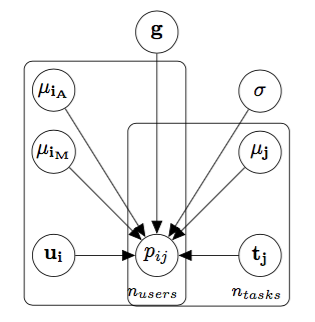
\includegraphics[height=8cm]{dgmaccurate.png}
  \caption{\label{fig:diagram} Model of prediction generation.}
\end{figure}
 
           
The good judgement matrix factorization model depends on an accurate estimation of various individual user parameters, requiring several predictions from a user before accurate predictions can be made. To mitigate these concerns, we use non-task psychological data to try to predict a users latent variables. This is easier than predicting a user's cluster as it leads to an intuitive distance metric for training, whereas trying to directly predict the user's cluster provides only a very hard binary classification task.

We focus only on the prediction of user latent vectors from non prediction data. Similar techniques could be used to solve the cold-start problem for tasks, however this would require data about tasks which come in before predictions. This is not part of the standard Good Judgement dataset and we did not explore feature engineering to create pre-prediction task data. An interesting direction for future work would be to consider natural language analysis techniques on text to create pre-prediction task data. For predicting the user latent variable models from psychological data, we try two separate techniques: 

\noindent\textbf{1. Predict latent variables from psychological data: } In our first model, we try predicting a user's latent variable representation directly from their psychological data. We use both a more interpretable simple linear regression model and a less interpretable fully connected neural network to perform the predictions. Then, it would be possible to make a prediction of a user's task report using a weighted combination of the predicted latent variables and the trained latent variables from matrix factorization. 

\noindent\textbf{2. Create user latent variable representation by summing feature latent variables} In this model, adapted from \citep{kula2015metadata}, a user's latent variable representation is created through a summation of various feature latent variables. If $f$ is a set of features, then each feature has a latent vector $\mathbf{L_{f}}$. Then for user $i$ with feature values $u_{if}$, the user's latent variable representation is $$u_{i} = \sum_{i=1}^{\vert f \vert} u_{if} \mathbf{L_{f}} + \mathbf{L_{u_{i}}}$$ where $\mathbf{L_{u_{i}}}$ is a user-specific latent vector which starts at $\mathbf{0}$. Then, predictions for a user start by using latent vector $\sum_{i=1}^{\vert f \vert} u_{f} \mathbf{L_{f}}$ only as the user-specific latent variable starts at $\mathbf{0}$. As data on the user comes in, the user-specific latent vector $\mathbf{L_{u}}$ moves away from $\mathbf{0}$. Predictions are then made as usual through  $$
  p_{i,j} = \textrm{tanh}\left( \mu_{i_M}\left[u_i^{T}t_j + g + \mu_j\right] + \mu_{i_A}\right)
 $$

\section{Training}\label{sec:training}

%\begin{itemize}
%\item How do you plan on training your parameters / inferring the
%  states of your latent variables (MLE / MAP / Backprop / VI / EM / BP / ...)
%
%\item What are the assumptions implicit in this technique? Is it an approximation or exact? If it is an approximation what bound does it optimize?
%
%\item What is the explicit method / algorithm that you derive for learning these parameters?
%\end{itemize}

For learning the latent user parameters, we use mini-batch stochastic gradient descent to find the maximum likelihood estimate. We choose not to use a prior for regularization as we find that the training and validation performance do not generally diverge. This is likely because there is already enough noise in the training data for each parameter that it is difficult to overfit the model. We do not explicitly code the initialization of the model, so of course it is possible it finds a local rather than global minimum. However, the performance of the model is consistent across random starts.

\begin{algorithm}
  \begin{algorithmic}
  \STATE {learning rate = $\alpha$}
  \FOR{\textrm{epoch in epochs} }
  \FOR{\textrm{batch in batches} }
    \STATE{Calculate the gradient of the MSE Loss for each parameter for all users and tasks in the batch}
    \STATE{Update the parameters: \\param $\gets$ param - $\alpha$ * $\frac{d}{dparam}$(MSE Loss) }    
    \ENDFOR
    \ENDFOR
  \end{algorithmic}
  \caption{Mini-Batch SGD Parameter Fitting}
\end{algorithm}

In the above algorithm, parameters include user and task specific biases, the global bias, the latent vectors for tasks, and the latent vectors for specific users as well as user features. In \citep{kula2015metadata}, the user feature latent vectors were trained at the same time as user specific latent vectors. However, for reasons described below, we find that it makes more sense to train  the latent variable model first only for user feature latent vectors. Then, after locking the user feature latent vectors and a corresponding set of task parameters: $t$, we then train a set of user specific latent vectors. Reports for new users are predicted as $$
  p_{i,j} = \textrm{tanh}\left(u_i^{T}t_{j} + g + \mu_{j} \right)
 $$ where $u_{i}$ is formed as described in Section \ref{ssec:non-task}. Reports for all other users are predicted as $$p_{i,j} = \textrm{tanh}\left( \mu_{i_M}\left[u_{i}^{T}t_{j} + g + \mu_j\right] + \mu_{i_A}\right)$$ The global bias $g$ and task-specific bias $\mu_{j}$ were allowed to vary throughout both training stages, although their values did not change much from stage 1 to 2. 

There are two reasons that we train the user feature vectors before the individual user biases. First, while the model incorporating user feature biases is clearly more general than vanilla matrix factorization, it has more parameters and can be sensitive to the learning rate. In particular, we found that training all at once provided a worse RMSE on the predicted report values than vanilla matrix factorization, with the former having a RMSE of 0.33 and the latter having an RMSE of 0.28. This is most likely due to a too high learning rate, but the model already takes a significant time to converge at the high learning rate. If we train the user feature vectors first, and then the individual user latent vectors, the final RMSE was 0.24. 

Additionally, the model above does not a unique global minimum. To see this, assume we are at some global minumum and there exists binary feature $f$. Then consider subtracting some $k$ dimensional vector $a_{k}$ from the feature latent vector $\mathbf{L_{f}}$ and then adding the same vector to each user latent vector $L_{u_{i}}$ with $u_{i}$ having feature $f$. Then, $u_{i} = \sum_{i=1}^{\vert f \vert} u_{if} \mathbf{L_{f}} + \mathbf{L_{u_{i}}}$ is the same for each user and so we still have the same globally minimum error. Thus, we seek to train our data in such a way that the user feature latent vectors are informative as possible. One way to achieve this is to train only the user feature latent variables first and minimize loss, and then to train the individual user latent vectors after. 


\section{Methods}

%\begin{itemize}
%\item What are the exact details of the dataset that you used? (Number of data points / standard or non-standard / synthetic or real / exact form of the data)

%\item What are the exact details of the features you computed?

%\item How did you train or run inference? (Optimization method / hyperparameter settings / amount of time ran / what did you implement versus borrow / how were baselines computed).

%\item What are the exact details of the metric used?
%\end{itemize}

For the \emph{Good Judgment} Dataset, we use the file \texttt{survey\_fcasts.yr4.tab}, consisting of all user forecasts for the fourth year of the tournament. The file has 1,685,784 lines, each consisting of details about a specific user id and forecast. We restrict to only binary valued questions, for which a single probability of `yes' is given as the answer (as opposed to, for example, ``Who will be inaugurated as President of Russia in 2012?", which had 3 possible answers). We restrict to only users who responded to at least 30 Individual Forecasting Problems (IFPs) over the course of the year. Given that users can (and ideally do) update their predictions for IFPs over time, any given time period could be thought of as a new IFP. Following the scoring procedure of the Good Judgment, we assume that if a user enters a prediction and then does not update it, this implies that they would like their existing prediction to be carried forward until they do update. We allow each week an IFP is active to be a different prediction task to balance temporal variability in task signals with our desire for higher task report density.

In computing the user latent vectors, we transform each prediction p from the range $[0,1]$ to $[-1, 1]$ via the transformation $$p = (p - 0.5) * 2$$. This puts the predictions over the entire range of the tanh function and makes it so the the multiplicative user bias smoothly transforms data towards predictions of $1$ or $-1$ (as opposed to outside the range). We train with stochastic gradient descent for 75 epochs with a learning rate of .2. 

\subsection{Clustering} As a metric of the clustering success, we use the average element-wise L1 distance between clustered $\Delta$ matrices and the original user-user $\Delta$ matrices for each pair of users. This requires binning the continuous predictions into discrete buckets. We choose to use 5 uniformly spaced bins from 0 to 1. We then compute the empirical joint distribution for any two users based on these discrete signals, as well as the empirical signal distributions of each individual. As mentioned in Section \ref{sec:Background}, the $\Delta$ matrices can be calculated from these as:
\begin{align*}
D_{q,r}(i,j) &= p(\textrm{q reports i, r reports j}) \\
&- p(\textrm{q reports i})p(\textrm{r reports j})
\end{align*}
To cluster, we use the scikit-learn implementation of K-means on all cores. The baseline we compare to is that of clustering on the $\Delta$ matrices directly, which is the method described in \citet{agarwal2017} and should in general be better at guaranteeing similarity of $\Delta$ matrices than clustering on other factors. In regards to user coordinates for clustering, we append all of the $\Delta$ matrices between that user and all other users, leaving NaNs where not enough data exists to compute a distribution, and flatten this into a vector. When clustering, we iteratively impute coordinate means for NaNs such that they are not taken into consideration in the clustering. 

The \emph{Adult} Dataset has 92,720 lines, each of which has a report by a user id on a website. Ratings are discrete and ordinal, and we use them as given for both learning latent user variables and for computing $\Delta$ matrices.

\subsection{Cold Start Problem}

As described in Section \ref{sec:training}, in the cold start problem we focus on predicting latent variables directly instead of on predicting clusters. In technique 1, we predict latent variables from labeled data coming from vanilla matrix factorization. So this takes as input the results of a complete matrix factorization, so that we have labeled data for each user of (user id, psychological data) $\times$ (latent vector representation). The first technique we tried was to perform simple linear regression over the psychological features onto the latent vector representations. In the second case, we trained a fully connected neural network. We tried 3 and 4 layers for the network, and varied the number of internal nodes between 20 and 80 for both layers. We found the best performance with a shallow network of just 3 layers and a middle layer of 20 nodes. Both techniques use out of the box PyTorch libraries. 

For the second technique of using user feature dependent latent vectors, we implemented the model using PyTorch. The model was then trained using stochastic gradient descent, with a learning rate of 0.2. We took 75 iterations to train the matrix factorization unless otherwise noted. 

\section{Results}

%\begin{itemize}
%\item What were the results comparing previous work / baseline systems / your systems on the main task?
%\item What were the secondary results comparing the variants of your system?
%\item This section should be fact based and relatively dry. What happened, what was significant?
%\end{itemize}


\begin{table}[t]
\centering
\caption{Distribution of L1 Distances Across Clusterings}
\label{fig:dist}
\begin{tabular}{lllll}
     & $\Delta$ (100) &K=2 (100) & $\Delta$ (500)  & K=2 (500)\\ \hline
\multicolumn{1}{l|}{mean} & .0168         & .0215   & .0145         & .0192   \\
\multicolumn{1}{l|}{std}  & .0243         & .0290   & .0218         & .0258   \\
\multicolumn{1}{l|}{min}  & 0             & 0       & 0             & 0       \\
\multicolumn{1}{l|}{25\%} & .0021         & .0043   & .0015         & .0036   \\
\multicolumn{1}{l|}{50\%} & .0084         & .0108   & .0071         & .0099   \\
\multicolumn{1}{l|}{75\%} & .0216         & .0271   & .0186         & .0244   \\
\multicolumn{1}{l|}{max}  & .7118         & .6864   & .6536         & .6191  
\end{tabular}
\end{table}

\begin{table}[t]
\centering
\caption{Runtime (s) of KMeans algorithm on User Representation}
\label{fig:time}
\begin{tabular}{lllll}
                         \multicolumn{1}{l|}{Clusters}& $\Delta$ & K=2 & K=3 & K=4 \\ \hline
\multicolumn{1}{l|}{100} & 423      & .57 & .55 & .65 \\
\multicolumn{1}{l|}{150} & 625      & .66 & .66 & .66 \\
\multicolumn{1}{l|}{200} & 800      & .66 & .77 & .87 \\
\multicolumn{1}{l|}{250} & 959      & .87 & .88 & .97 \\
\multicolumn{1}{l|}{300} & 1187     & .96 & 1.1 & 1.1 \\
\multicolumn{1}{l|}{350} & 1198     & 1.1 & 1.2 & 1.2
\end{tabular}
\end{table}

\begin{table}[t]
\centering
\caption{Cold Start Predictions}
\label{tbl:cold_start_technique_1}
\begin{tabular}{lllll}
                         \multicolumn{1}{l|}{Method}& Mean Distance \\ \hline
\multicolumn{1}{l|}{Baseline (Mean Latent Vector)} & 0.67 \\
\multicolumn{1}{l|}{Linear Regression} & 0.58 \\
\multicolumn{1}{l|}{Neural Network} & 0.56 \\

\end{tabular}
\end{table}
\subsection{Sophie}
While we achieved the lowest training and validation loss using 10 latent user factors (See Figure~\ref{fig:train}), the best L1 loss against the original $\Delta$ matrices was achieved by clustering on only 2 latent user factors (See Figure~\ref{fig:clust_dist}).  Distribution results are given in Table~\ref{fig:dist}.

However, clustering on the latent factors for all values of K was significantly faster than clustering directly on the $\Delta$ matrices, as the flattened concatenated matrices result in 51,300 features for each user. See Table~\ref{fig:time} for details.

\subsection{Cold Start Problem: Predicting Latent Variables Directly} Table \ref{tbl:cold_start_technique_1} shows the performance using a Neural Network and simple linear regression in predicting the latent variables for new users from just psychological data. The mean distance is calculated as the $\ell_{2}$ distance from their final trained values after observing predictions and updating their latent vectors. Both are compared to just using a latent vector made up of coordinate-wise mean values for each new user. That is, the mean vector takes each of the $k$ dimensions for a latent vector and estimates a new user's value in that dimenion by the average of every other user's value for that dimension. 

For both linear regression and the neural network, there is some improvement over just using the mean latent vector, and so we see some improvement over a random guess for new users. Ideally, this effect would be much larger; the extent to which this is possible using the psychological data for Good Judgment is unknown. Indeed, considering that there was no prior method of predicting new user's reports for Good Judgment, this provides some utitlity.

\begin{table}[t]
\centering
\caption{Cold Start Predictions}
\label{tbl:LightFM}
\begin{tabular}{lllll}
                         \multicolumn{1}{l|}{Method}& Mean Distance \\ \hline
\multicolumn{1}{l|}{Baseline (Mean Latent Vector)} & 0.61 \\
\multicolumn{1}{l|}{From Sum of User Feature Vectors} & 0.53 \\

\end{tabular}
\end{table}

Table \ref{tbl:LightFM} shows the results for a similar experiment using the feature-based expansion of matrix factorization. In this second set of results, we look at a user's initial latent vector from its features and calculate the $\ell_{2}$ distance from its final latent variable $u_{i}$ after training. Similarly to before, we compare this to using the mean latent vector for a user. We note that this is not in the same table as Table \ref{tbl:cold_start_technique_1} because the corresponding set of task latent vectors is different. 

\section{Discussion}



%\begin{itemize}
%\item What conclusions can you draw from the results section?
%\item Is there further analysis you can do into the results of the system? Here is a good place to include visualizations, graphs, qualitative analysis of your results.

%\item  What questions remain open? What did you think might work, but did not?
%\end{itemize}

The results show us that it is possible to use a significantly compressed representation of user heterogeneity and still arrive at a clustering that is still almost as successful at encouraging truthful reporting as the significantly more time- and memory-intensive task of clustering directly on the user-user signal distributions. Notably, the user representation we use does not explicitly encode the interactions between any two users` reporting behaviors yet performs nearly as well as the clustering will full knowledge of this data.

We note that the RMSE and L1 loss of the training model are lowest for larger numbers of latent factors, yet the clustering performs best when only two latent factors are used. One possible explanation is that this setup forces more of the user variability into the multiplicative and additive biases, which are more specifically relevant to the task of predicting a distribution of reports given signals. Supporting this interpretation, clustering the \emph{Adult} dataset, which does not have the task structure to allow for modeling known psychological biases (specifically with respect to probability reporting) as its latent user biases, does not degrade as we increase the number of latent factors.

TODO INCLUDE CHART

\begin{figure}
  \centering
  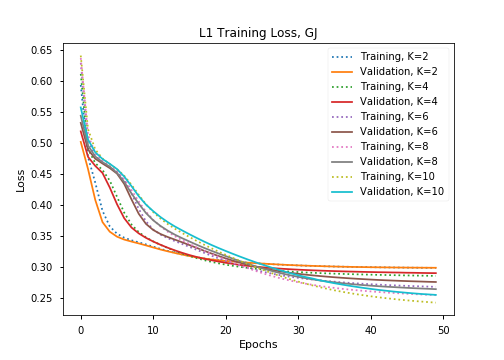
\includegraphics[width= \columnwidth]{training.png}
  \caption{\label{fig:train} Training Results, L1 Loss.}
  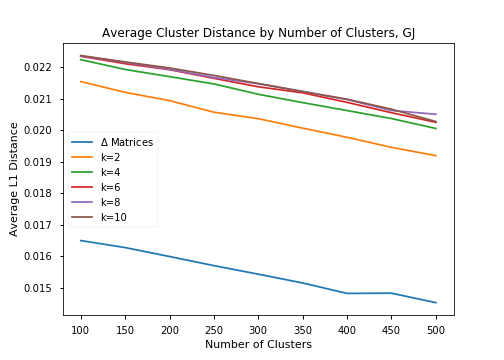
\includegraphics[width= \columnwidth]{clust_dist.png}
  \caption{\label{fig:clust_dist} Average L1 Distance.}
  \missingfigure{}
  \caption{Visualizations of the internals of the system.}
\end{figure}

\section{Conclusion}

\begin{itemize}
\item What happened?
\item What next?
\end{itemize}

\lipsum[4-6]

% \section*{Acknowledgements}

% \textbf{Do not} include acknowledgements in the initial version of
% the paper submitted for blind review.

% If a paper is accepted, the final camera-ready version can (and
% probably should) include acknowledgements. In this case, please
% place such acknowledgements in an unnumbered section at the
% end of the paper. Typically, this will include thanks to reviewers
% who gave useful comments, to colleagues who contributed to the ideas,
% and to funding agencies and corporate sponsors that provided financial
% support.


\bibliography{example}
\bibliographystyle{icml2017}

\end{document}
